\section{Hybrid Recommender System}
In this section, we will demonstrate the implementation of a hybrid system that combines matrix factorization and the content-based approach.

\textbf{\textit{Dataset}}. To verify the generality of the system, in addition to the MovieLens dataset we have used in the user-based system, we will also use a dataset called Jester\footnote[4]{Dataset available at: http://eigentaste.berkeley.edu/dataset} which contains over 1.7 million continuous ratings (-10.00 to +10.00) of 150 jokes from 59,132 users.

\textbf{\textit{Recommendation}}. Based on the method and implementation of matrix factorization described above, we can get our user latent matrix \textit{p} and item latent matrix \textit{q}. By performing the inner product between the above two latent matrices, we get the predicted user-item rating matrix $\hat{R}$. For the example shown in Figure 4.20, if we want to get the predicted rating of user 1 on item 1, we can use the inner product between two matrices to get the predicted rating. The process is shown in (a), and the predicted rating here is 3.999. When compared with the grand true rating shown in (b), we can see that the approximation of the predicted rating to the true rating is 99.975$\%$.

\begin{figure}[htbp]
\centering
\subfigure[Predicted rating]{
\begin{minipage}[t]{0.5\linewidth}
\centering
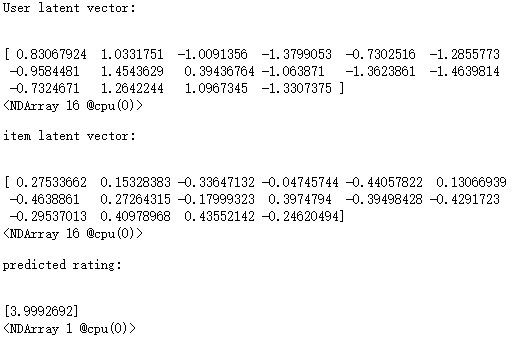
\includegraphics[scale=0.6]{figure/h1.png}
%\caption{fig1}
\end{minipage}%
}%
\subfigure[Grand true rating]{
\begin{minipage}[t]{0.5\linewidth}
\centering
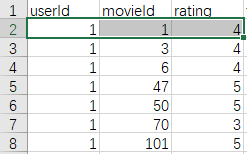
\includegraphics[scale=1]{figure/movie6.png}
%\caption{fig2}
\end{minipage}%
}%
\centering
\caption{comparison between predicted rating and true rating }
\end{figure} 

As per the methods that we talk about in section 3.3, the next step is to sort the movies that have not been rated by the target user through our predicted rating score and recommend the top-ranked movie to the target user. Through Figure 4.21, we can get the information that a movie with ID 910 is the movie with the highest predicted rating. 
\begin{figure}[htbp]
\centering
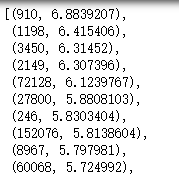
\includegraphics[scale =1]{figure/h2.png}
\caption{Top 10 movies with high predicted rating}
\end{figure}

\textbf{\textit{Content-based recommendation}}. By the movie ID, we know that this movie is called \textit{``Some Like It Hot (1959)''}. All that is left for the hybrid recommendation system to do is to suggest movies similar to the movie \textit{``Some Like It Hot (1959)''} to the target user. 

Like what we described before, in order to measure how similar the movies are in attractiveness to the target user, we need to calculate the similarity by some formula. To test the ability of different similarity formulas, different from the \textit{Pearson Correlation Coefficient} used in the previous user-based system, we use \textit{Cosine similarity} to calculate the similarity, where the following formula can be used to calculate the similarity between movie $i$ and movie $j$:
\begin{equation}
\operatorname{similar}(i, j)=\cos (i, j)=\frac{i \cdot j}{\|i\| \cdot\|j\|}
\end{equation}
Figure 4.22, (a) shows the top 10 movies that are similar to the movie \textit{``Some Like It Hot (1959)''}. In (b), if we want to recommend two more movies to the target user, as the recommendation result of this hybrid system, movie \textit{`` The Fate of the Furious (2017)’’} which ID is 170875 and movie \textit{`` Withnail $\&$ I (1987)’’} which ID is 1202 will be recommended to the target user who likes the movie \textit{``Some Like It Hot (1959)''}.

\begin{figure}[htbp]
\centering
\subfigure[Top 10 items with high similarity]{
\begin{minipage}[t]{0.5\linewidth}
\centering
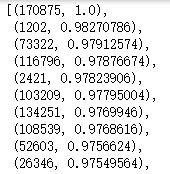
\includegraphics[scale=1]{figure/h3.png}
%\caption{fig1}
\end{minipage}%
}%
\subfigure[Recommendation result]{
\begin{minipage}[t]{0.5\linewidth}
\centering
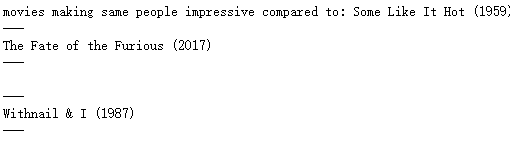
\includegraphics[scale=0.65]{figure/h4.png}
%\caption{fig2}
\end{minipage}%
}%
\centering
\caption{Content-based recommendation}
\end{figure} 

\begin{figure}[htbp]
\centering
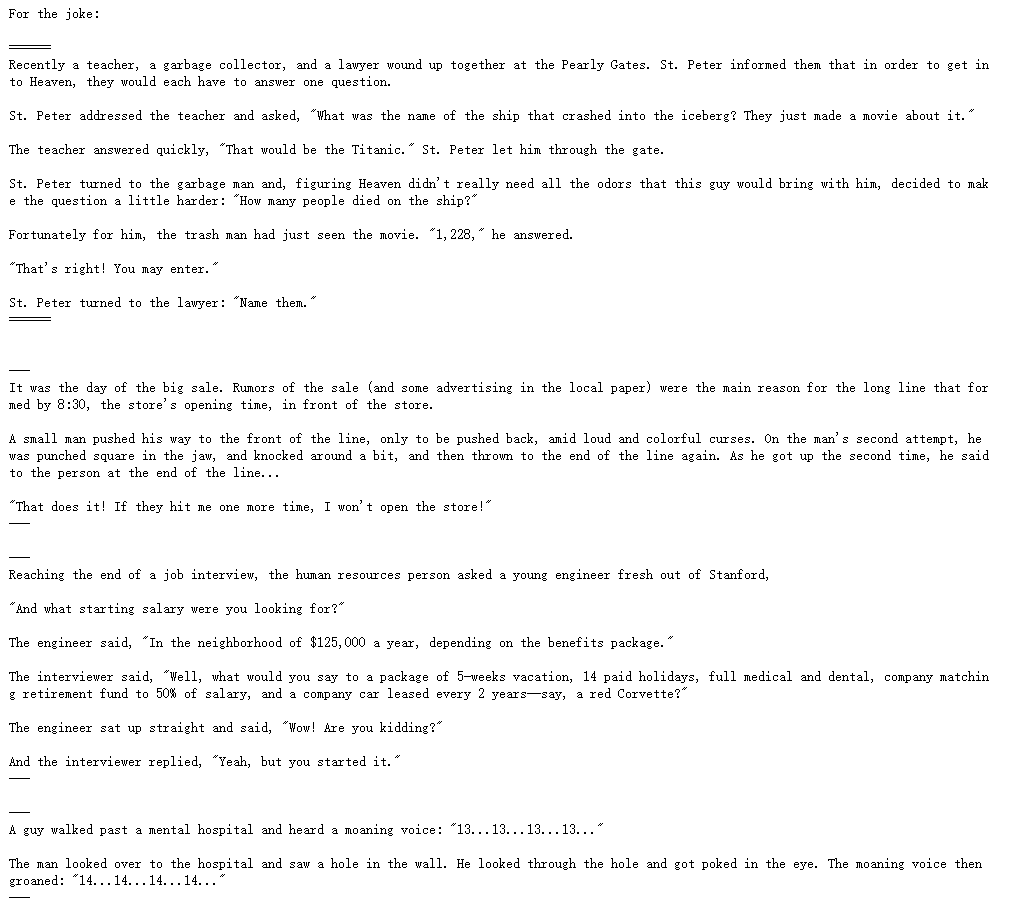
\includegraphics[scale =0.47]{figure/h5.png}
\caption{Joke recommendation}
\end{figure}

When we repeated the above steps on another dataset, Jester on Jokes, our results are shown in Figure 4.23. By matrix factorization, we get the most recommended jokes for the target user (bounded by double lines), and based on content-based recommendations, three jokes similar to the matrix factorization recommended jokes are derived (bounded by signal line).